\documentclass[]{article}
%\usepackage{euler}
\usepackage{amsmath}
\usepackage{amsfonts}
\usepackage{amssymb}
\usepackage{mathtools}
\usepackage{graphicx}
\usepackage{url}
\usepackage{listings}
\usepackage[utf8]{inputenc}
\usepackage[english]{babel}
\usepackage{framed}
\usepackage[most]{tcolorbox}
\usepackage{courier}



\newtheorem{theorem}{Theorem}

\newtheorem{benexample}{Example}

\newcommand{\Z}{\mathbb{Z}}
\newcommand{\OS}{\mathbb{O}}
\newcommand{\ZMZ}[1]{\Z/#1\Z}
\newcommand{\Q}{\mathbb{Q}}
\newcommand{\F}{\mathbb{F}}
\newcommand{\R}{\mathbb{R}}
\newcommand{\Mod}[1]{\ (\text{mod }#1)}
\newcommand{\kf}{\bold{k}}
\newcommand{\floor}[1]{\lfloor #1 \rfloor}
\newcommand{\ceil}[1]{\lceil #1 \rceil}
\newcommand{\leg}[2]{\Big( \frac{#1}{#2} \Big)}

\graphicspath{ {projpics/} }


%opening

\title{Primality Certification with Elliptic Curves}
\author{Ben Black}

\begin{document}
\lstset{language=Python}

\maketitle

\section{Primality Testing and Certification}

In modern day cryptography, the Miller-Rabin probabilistic primality test is universally used for checking primality of general integers. It is much faster both practically and algorithmically than any deterministic primality test, for any reasonable bound on certainty. In fact, if we set our reasonable bound of certainty to that of a hardware failure giving us an incorrect answer, then it is still much, much faster. Because the chance of hardware failure increases with increased computation time and memory usage, it can be argued that Miller-Rabin can actually give a more certain result than some deterministic tests.

So how can general purpose deterministic primality tests prove their worth in this imperfect world? The way I will discuss in this paper is the ability to generate short, easily checkable proofs of primality, which can be verified much faster using much simpler code than the generator of the proof. Even if this process of finding the proof is fairly slow, then being able to check them may still have potential uses.

\begin{itemize}
	\item If you are using an internet service which generates primes, and you don't like the certainty guarantees of checksums to validate that there were no errors in the transfer, then you could send both the prime, and the proof of the prime, and verify the proof on on site.
	\item If you wanted to store large databases of provable primes and didn't trust that the storage hardware would keep them correctly, you could also store the proof of the prime, and just check it whenever you need to use the prime. 
\end{itemize}

The best algorithm for finding such a proof of primality is ECPP, the elliptic curve primality test discovered by Atkin and Morain. Although far slower than Miller-Rabin, it is fast enough to operate on cryptographically important primes in a few seconds. Unfortunately, ECPP is quite complicated and well beyond the scope of this paper. However, the condition one needs to check the primality certificate it generates is quite simple, just based on clever analysis of orders in elliptic curves. I will introduce the theory of an elementary version of the certificate the Pocklington criterion, then the elliptic curve primality criterion, show a simple algorithm to generate these checks for arbitrary primes, and then argue that these may be useful in real world applications.

\section{Pocklington primality test}

The elliptic curve primality condition is modeled after the Pocklington primality test. I will explain it here in order to give some extra intuition.

\subsection{Inspiration}

Fermat's little theorem states that for $p$ prime, and $a$ coprime to $p$, $$a^{(p-1)}=1 \Mod{p}$$ We wish to find a converse to this statement that gives some set of conditions that force primality. To start, we know that $(p-1)$ is the smallest power of $a$ that equals 1. Also, for $m$ composite, we know that $a^{l}=1 \Mod{p}$ for some $l < p-1$. Specifically, we can use the fact that $(\ZMZ{p})^*$ is cyclic to give the following statement.

\begin{theorem}
	If there exists an $a$ coprime to $n$ such that $a^{n-1} = 1 \Mod{n}$ but $a^{(n-1)/q} \ne 1 \Mod{n}$ for every prime $q | n-1$, then $n$ is prime.
\end{theorem}

%(EXAMPLE OF THIS CONDITION IN ACTION!!!!!!!!!!!!!!!!!!!!!!!!!!!!!!!!!)

We now have a condition for primality. However, there is the problem that we need to factor $n-1$, which is not generally computationally tractable. However, if we already knew factors, then we could easily and quickly verify the primality of $n$ by the above condition.
So the certificate of primality of $n$ would simply be the factorization of $n-1$.


\subsection{Pocklington Criterion}

%http://blog.fkraiem.org/2013/04/08/primality-testing-part-2-the-pocklington-lehmer-primality-test/
Pocklington's insight was that if there was a large prime factor $q$ of $n-1$, then there are some conditions that allow us to show primality only based on the primality of $q$, and even if we don't know the other factors of $n-1$. Formally,

\begin{theorem}
Let $n > 1$ be an integer, $q$ a prime divisor of $n-1$, and $a$ coprime to $n$.
%https://en.wikipedia.org/wiki/Pocklington_primality_test#Proof_of_this_theorem
%
If $$q > \sqrt{n}-1$$ and $$\gcd(a^{(n-1)/q}-1,n) = 1$$
%
Then $n$ is prime
\end{theorem}

\subsection{Proof of Pocklington Criterion}

%https://en.wikipedia.org/wiki/Pocklington_primality_test#Proof_of_this_theorem

Suppose $n$ is composite. Then there must be a $p \le \sqrt{n}$ that divides $n$.

We are going to look at the order of $\F_p$ which is, $p-1$, to reach a contradiction.

We have
%http://blog.fkraiem.org/2013/04/08/primality-testing-part-2-the-pocklington-lehmer-primality-test/
$$a^{n-1} = 1 \Mod{p}$$
Since $q$ is prime, and $q > \sqrt{n}-1 \ge p-1$, $q$ is coprime to $p-1$. Therefore, $q$ is multiplicatively invertible in $(\ZMZ{(p-1)})^*$, and so we can just multiply the exponent of $a$ by the inverse of $q$
$$(a^{(n-1)})^{1/q} = a^{(n-1)/q} = 1 \Mod{p}$$
Which contradicts the condition $\gcd(a^{(n-1)/q}-1,n) = 1$. So $n$ is prime.

\subsection{Proof Certificate using Pocklington's Criterion}

Note that factoring $n-1$ is trivial if it factors into $2p$, where $p$ is prime.
Also note that we get the size condition of Pockington's criterion, $p > \sqrt{n}-1$, for free because is $p$ such a large factor of $n-1$. 

Understanding that not all $n$ are of this sort, we can still use Pockington's criterion to say that if $\gcd(a^{(n-1)/q}-1,n) = \gcd(a^2-1,n) = 1$, and that $p$ is prime then $n$ is prime. Of course you need to check if $p$ is prime, but hopefully you can use the same method to check that. And so on until you create a decreasing chain of primes
$$n > p_0 > p_1 > ... > p_{small}$$
that demonstrate the previous number's primality.

\begin{tcolorbox}[breakable,
	enhanced,
	standard jigsaw,
	opacityback=0]
	
	\noindent \begin{benexample}
		Creating a full proof of primality for $n=47$,
	\end{benexample}
	
	\begin{tabular}{ l | c | r }
		$n$ & $q=(n-1)/2$ & $\gcd(a^2-1,n)$ \\
		\hline
		47 & 23 & 1\\ \hline
		23 & 11 & 1\\ \hline
		11 & 5 & 1\\ \hline
		5 & 2 & 1\\ \hline
		
	\end{tabular}
	
	\noindent 2 is clearly prime, so each $n$ is in turn prime, and so 47 is prime.
\end{tcolorbox}


Even though this method does not work for general primes, we will make a similar method work using elliptic curves. The key will be that although there is only one $(\ZMZ{n})^*$, there are many elliptic curves over $\ZMZ{n}$, and some of them will have order $2p$, where $p$ is prime.

\section{Elliptic Curves Overview}

\subsection{Introductory Sources}

There are many fabulous introductions to the basics of elliptic curves, including

\begin{itemize}
	\item The fabulous explanation by Andrea Corbellini. It includes interactive components and a thorough overview that does not require much background in algebra. Posted here:

	\url{http://andrea.corbellini.name/2015/05/17/elliptic-curve-cryptography-a-gentle-introduction/#elliptic-curves}
	\item Joseph H. Silverman
	John T. Tate
	Rational
	Points on
	Elliptic Curves
\end{itemize}

As these are better written than I could ever manage, I not attempt to introduce elliptic curves in a comprehensive manner, especially since most of the theory is unnecessary for our purpose. Instead, I will just cover the important topics such as order of elliptic curves.

\subsection{Refresher}

Recall that elliptic curves are defined in a plane of $\F^2$, where $\F$ is some field, as formulas 

$$y^2 = x^3 + ax + b \text{ where }a, b \in \F$$

There is a group operation $+$, with identity $\OS$ which is an additional point on the elliptic curve that is not on the plane. It is often referred to as the point at infinity. You can add points $(x_1,y_1)$ and $(x_2,y_2)$ on elliptic curves by the formulas 

\[
m = \left\{\begin{array}{lr}
\frac{y_2-y_1}{x_2-x_1}, & \text{if } x_1 \ne x_2 \\
\frac{3x_1^2+a}{2y_1}, & \text{if } x_1 = x_2
\end{array}\right\}
\]

$$x_r = (m^2-x_1 - x_2)$$
$$y_r = -(y_1 + m(x_r - x_1))$$

\noindent And $(x_r,y_r)$ is the result.

Finally, multiplication of a point by an integer $m$ is repeated addition of the point by itself $m$ times. 

\subsection{Calculating Elliptic Curve Arithmetic}

Calculating these formulas is difficult and error prone to work out by hand, and is not pleasant even using an ordinary calculator. I wrote a python file to support this paper, and in it is an \texttt{add} function and a \texttt{mul} function to help calculate addition and multiplication of elliptic curves.

It can be found here: \url{https://github.com/weepingwillowben/num_proj/blob/master/prime_check.py}. 
It uses the gmpy2 math library for modular arithmetic, and so unfortunately, it is non--trivial to install. Installation instructions are at the top of the file. All elliptic curve examples shown were made using this code to calculate operations.

\subsection{Note about $E(\ZMZ{n})$}

Now that we are getting into the main subject of the paper, I have to mention a problem with elliptic curves in these sorts of proofs. That is, elliptic curves are only well defined over fields, and $\ZMZ{n}$ is not a field unless $n$ is prime. However, it turns out to not be too much of a problem, as operations work as you might expect them to, if they are well defined.

In particular, let $L,M \in E(\ZMZ{n})$. Define $L_p = (x_p,y_p) \in E(\F_p)$, and $\OS_p = \OS \in E(\F_p)$. Then if $L+M$ is defined, then $(L+M)_p = L_p + M_p$.

So how do we check if the group operation is well defined? Recall the formula for the slope of the line

\[
m = \left\{\begin{array}{lr}
\frac{y_2-y_1}{x_2-x_1}, & \text{if } x_1 \ne x_2 \\
\frac{3x_1^2+a}{2y_1}, & \text{if } x_1 = x_2
\end{array}\right\}
\]

This operation fails in $\ZMZ{n}$ if the denominator of the respective formula is not invertible $\Mod{n}$. This occurs exactly when

\[
\left\{\begin{array}{lr}
\gcd(x_2-x_1,n), & \text{if } x_1 \ne x_2 \\
\gcd(2y_1,n), & \text{if } x_1 = x_2
\end{array}\right\}
\ne 1
\]

It turns out that $\ZMZ{n}$ is near enough to a field that this is the only way in which the elliptic curve assumptions fail, so this is an if and only if.

In the context of factoring and primality proving, the failure of addition reveals that $n$ is not prime, and in fact, gives a factor of $n$, and so we don't have to continue to try to work in $\ZMZ{n}$ anymore. So the failure condition for addition in $E(\ZMZ{n})$ actually helps our work, instead of limiting us.


\section{Elliptic Primality Testing}

\subsection{Approach}

For the Pocklington criterion, we examined the order of the cyclic group $(\ZMZ{p})^*$ in order to prove primality. In $(\ZMZ{n})^*$, the order is $(n-1)$. So we look at the order of elliptic curves in order to find a similar result.

\subsection{Orders of Elliptic Curves}

\subsubsection{Theory}
The order of a point on an elliptic curve, denoted $\#L$, is the number of times you can add a point $L \in E_{A,B}(\F_p)$ to itself before getting back the identity $\OS$. Formally, $\#L$ is the smallest $m$ such that $mL = \OS$. Note that this implies that if you multiply $L$ by $m+1$, you get back $L$, and $(m+2)L = 2L$, and so on, and so you can think of the multiplicand operating in $\ZMZ{m}$. This is a special case of the fundamental theorem of finite abelian groups. Alternatively, $mL = \OS$ can be though of as Fermat's little theorem for elliptic curves. Order analysis on points forms the basis for the primality test, mirroring Pocklington's criterion.

Order on the curve itself is defined very differently. 
For $E_{A,B}(\F_p)$, the order of an elliptic curve, denoted $\# E_{A,B}(\F_p)$ is the number of points in the elliptic curve. For any $L \ne \OS \in E_{A,B}(\F_p)$, $\# L$ divides $\# E_{A,B}(\F_p)$. 

\subsubsection{Algorithm}

It turns out that you can compute $\# E_{A,B}(\F_p)$ by counting the number of points on the elliptic curve in $\F_p^2$, plus the point at infinity. For a small $p$, one can count the points by just looking at the formula

$$y=\pm \sqrt{x^3+ax+b}$$

And checking counting how many times $y$ is an integer for all values $x \in \F_p$.

\begin{tcolorbox}[breakable,
	enhanced,
	standard jigsaw,
	opacityback=0]

	\noindent \begin{benexample}
		Counting points in $E_{1,1}(\F_5)$,
	\end{benexample}

	\noindent We have $x = 0,1,2,3,4$, and so $x^3+x+1 = 1,3,1,1,4$, respectively.

	\noindent The numbers which are quadratic residues, i.e. have a non-zero square roots in $\F_5$ are 1 and 4. So we have 4 values of $\pm y$, each of which non-zero, and so are distinct. So we have 8 points in total, 9 including $\OS$.

	\noindent So $\# E_{1,1}(\F_5) = 9$.
\end{tcolorbox}

Lets check the above theorem that the order is exactly the number of points on the curve.

\begin{tcolorbox}[breakable,
	enhanced,
	standard jigsaw,
	opacityback=0]

	\noindent \begin{benexample}
		Checking that point order divides number of points in $E_{1,1}(\F_5)$,
	\end{benexample}

	\noindent Take $(0,1) \in E_{1,1}(\F_5)$. Then perhaps using the point addition calculator here: \url{https://cdn.rawgit.com/andreacorbellini/ecc/920b29a/interactive/modk-add.html}, we can compute that

	\noindent $(0,1)+(0,1) = (4,2)$

	\noindent $(4,2)+(0,1) = (2,1)$

	\noindent $(2,1)+(0,1) = (3,4)$

	\noindent $(3,4)+(0,1) = (3,1)$

	\noindent $(3,1)+(0,1) = (2,4)$

	\noindent $(2,4)+(0,1) = (4,3)$

	\noindent $(4,3)+(0,1) = (0,4)$

	\noindent $(0,4)+(0,1) = \OS$


	\noindent Which is equal to $9 \times (0,1)$, so we confirmed that $\# (0,1) = 9\ |\ 9$, as desired.

\end{tcolorbox}

This counting algorithm is impractical if $p$ is large. Luckily, we have polynomial time algorithms for this, Schoof's algorithm, and it's variants and improvements. So this is a tractable problem. However, Schoof's algorithm is extremely complicated, as well as rather slow, so I will not cover it here.

\subsection{Bounds on Orders of Elliptic Curves}

Although counting precisely how many points are on a particular curve is a challenge, Hasse discovered useful bounds for it.

In particular, for $N$ the number of points on an elliptic curve over $\F_q$,
%https://en.wikipedia.org/wiki/Hasse's_theorem_on_elliptic_curves
$$|N-(q+1)| \le 2\sqrt{q}$$

We will use this in order to derive a contradiction that will prove the primality of $N$.

\subsection{Elliptic Primality Criterion}

We are going to use this order exactly like we used $n-1$ in the $(\ZMZ{p})^*$ based primality proof, and establish a nearly identical criterion.

\noindent \begin{theorem} Let $n$ be an integer not divisible by 2 or 3. Let $A,B \in \ZMZ{n}$ such that $\gcd(4A^3+27B^2,n) = 1$, and let $L \ne \OS \in E_{A,B}(\ZMZ{n})$. If there exists a prime $q > (\sqrt[4]{n}+1)^2$ such that $qL = \OS$, then $n$ is prime.
\end{theorem}

\begin{tcolorbox}[breakable,
	enhanced,
	standard jigsaw,
	opacityback=0]	
	\noindent \begin{benexample}
		Checking primality of $103$
	\end{benexample}
	
	Lets take $L = (85,81) \in E_{A=72,B=93}(\ZMZ{103})$. Then we can calculate that $53\times L = \OS$, and so by the theorem, 103 is prime if 53 is prime. 
	
\end{tcolorbox}


\subsection{Proof}

Proof by contradiction, assume some prime $p | n$. Mirroring the Pocklington criterion proof, we are going to look at the order of $L_p \in E_{A,B}(\F_p)$, which is the point $L$ defined over $\F_p$ instead of $\ZMZ{n}$.


\begin{enumerate}
	\item   $\gcd(4A^3+27B^2,n) = 1$ ensures that the elliptic curve is well defined over $E_{A,B}(\F_p)$, even though we don't know $p$, because if $p | 4A^3+27B^2$, then $p | \gcd(4A^3+27B^2,n)$.
	\item The $n$ does not divide 2 or 3 is going to be necessary for a later theorem that we need to show that we can actually find such an elliptic curve in polynomial time. But it isn't necessary for the criterion.
\end{enumerate}

\noindent Now the meat of the proof, using the notation from the $E(\ZMZ{n})$ section of the paper.

\noindent $qL_p$ = $(qL)_p$, by the elliptic curve behavior over $\ZMZ{n}$.

\noindent $qL = \OS$ by the criterion, and so $qL_p = \OS_p = \OS$, again by behavior over $\ZMZ{n}$.

\noindent  But since $L_p \ne \OS$ and $q$ is prime, the order of $L_p$ must be $q$. After all, if it were a number $t$ smaller than $q$ then we could talk about $qL$ in terms of $q \Mod{t}$, due to the fundamental theorem of albelian groups, where $0 \Mod{t}$ maps to $\OS$. But $q$ is coprime to $t$, so $q$ couldn't be 0, and so $qL$ couldn't be $\OS$ unless $t=1 \implies L_p = \OS$. But that is not true, by assumption. So indeed, the order of $L_p$ must be $q$. %(EXPLANATION NEEDED!!!!!!!!!!!!!!!!!)

\noindent But by Hasse's bound on the order of elliptic curves,

$$\begin{aligned}\# L_p &\le \# E_{A,B}(\F_p) & \text{ Definition of order on } L_p\\
 &\le (\sqrt{p}+1)^2  & \text{  Hasse's bound}\\
 &\le (\sqrt[4]{n}+1)^2 & \text{ Condition on } p\\
 &< q & \text{ Condition on } q\\
 \end{aligned}$$

\noindent  Which is a contradiction, so $n$ must be prime.

\subsection{Chains of Conditions}

Like I showed earlier with the Pocklington Criterion, these conditional proof of primality based on a smaller number's primality can be chained together to create a complete certificate of primality.

\begin{tcolorbox}[breakable,
	enhanced,
	standard jigsaw,
	opacityback=0]
	
	\noindent \begin{benexample}
		Checking that point counting and order are equivalent in $E_{1,1}(\F_5)$,
	\end{benexample}
	
	We can extend the example from before to also include the conditions that show that 53 is prime.
	
	\begin{tabular}{ c | c | c | c | c | c }
		$n$ & $L$     & $A$ & $B$ & $q$ & $qL$ \\ \hline
		103 & (85,81) & 72 &  93 &  53 &  $\OS$ \\ \hline
		53 & (4,30)   & 37 & 52 & 29  & $\OS$ \\ \hline
	\end{tabular}
	
	\noindent Now, we can easily check that 103 is prime if 29 is prime using the criterion.
	
\end{tcolorbox}

\subsection{Implementation}

Included in the my python code is a \texttt{check\_prime} function that takes in a curve, point, assumed prime, and number to check and outputs whether it is prime using the method described above. If you are good with code, you should be able to play around with it and see that it works exactly as described above. There is also a \texttt{check\_certificate} that checks a list of such information. 

\section{Generating the Primality Proof}

The ability to check this condition would not be useful in a practical setting unless we had the ability to generate the proof conditions for general numbers in polynomial time. There are two main ways of finding the curves and points which meet the criterion. The first one, the Goldwasser--Kilian algorithm, is much simpler, and so that is what I will describe in depth. The second one is much faster and is what is used in practice, but also much more complicated.

\subsection{Goldwasser-–Kilian Algorithm Overview}

This algorithm is based on guess and check. Naively, We want to just guess a curve, a point $L$, and large prime $q$ such that $qL = \OS$. In this algorithm, we will still end up guessing the curve and the point, but instead of finding the prime by guessing, we can use the relationship between point counting and order and do fast point counting using Schoof's algorithm in order to find our candidate $q$.

Choose $L$, a random point on  $\ZMZ{n}$, and choose a random elliptic curve $E$ over $\ZMZ{n}$, such that $L$ is in $E$. Count the number of points $m$. Check if $m$ satisfies $2q$, with $q$ a probable prime (checking with Miller-Rabin). Also check that $qL = \OS$. If both hold, then you have found the point, curve, and prime number that satisfy the condition.


\subsection{Implementation}

To make this more concrete, I made a really inefficient version of this algorithm based on the description in \underline{An Overview of Elliptic Curve Primality Proving} by Frank Li \cite{StanfordAlgo}.

The \texttt{gen\_and\_check\_certificate} function prints out the certificate and then checks it. It uses an exponential time point counting function instead of Schoof's algorithm, and an exponential time modular square root algorithm, so it unfortunately doesn't work on large primes, but hopefully it can be of use and maybe some fun.


\subsection{Distribution of Orders of Random Elliptic Curves}

%http://theory.stanford.edu/~dfreeman/cs259c-f11/finalpapers/primalityproving.pdf

At this point you might wonder how we know that we can find elliptic curves of the desired form. Perhaps we have the same problem as we had with Pockington's criterion, and we just described a special purpose primality proving algorithm. Or perhaps it takes too long to randomly find them.

It turns out that this really does work, though. The proof that there will always be an elliptic curve that we can find in expected polynomially many guesses is the following theorem due to Lenstra:

\begin{theorem}
Let $p \ne 2,3$ prime, and let $S \subseteq \{p+1 - \floor{\sqrt{p}},.., p+1 + \floor{\sqrt{p}}\}$. Let $A$,$B$ be  chosen from a uniform random distribution over $\F_p$. Then there exists fixed constants $k$ such that

$$Prob(\# E_{A,B}(\F_p) \in S) > \frac{k}{log(p)} \frac{|S|-2}{2 \floor{\sqrt{p}}+1}$$
\end{theorem}

\section{Real World Considerations}

For all practical purposes, the Primo software by Marcel Martin is the best available elliptic curve primality prover implementation for general numbers. Although the algorithm it uses to generate primality certificates is quite complicated, the certificate itself, and the method of checking it are both quite simple. It only requires a little more mathematical theory than in this paper, and only a couple hundred lines of code using a good math library like gmpy2. In fact, several people have actually created independent checks for Primo's certification files, although I have yet to find any that actually work on the most recent version of Primo. By pairing this independent checking with Primo's builtin verification, one should be able to rule out implementation errors or hardware failures with a very high confidence level, easily on par with that of a thorough Miller--Rabin test.

These checks should also be extremely fast. Assuming that the Primo checker is not taking incorrect shortcuts when verifying the certificate, we should be able to evaluate it's performance checking the certificates as the actual speed of checking primality. On my machine, using all cores, generating the proof of primality for the prime $(10^{1999} + 7321)$ took 678s. But checking the certificate only took $0.13$ seconds. For comparison, gmpy2's \texttt{is\_prime} function, which uses Miller--Rabin,  took 0.62 seconds for 6 runs of Miller--Rabin (the lowest end of reasonable confidence) and 1.69 seconds for 25 runs (the default). As gmp is well regarded as a high quality, fast library, and gmp's \texttt{mpz\_probab\_prime\_p} (which gmpy2's \texttt{is\_prime} uses) is actually used in some real world cryptographic applications, I think it fair to say that checking these elliptic curve primality certificates can be at least as fast, if not faster than a decent Miller-Rabin test. 

So hopefully I have shown how deterministic primality testing may have some use in practical applications as well as explaining the basic theory enough to explore the topic with some more comfort.


%Primo certificate generation: 678s (all cores)
%Primo certificate check: 0.13 seconds

%gmpy2 primality check 1 pass: 0.15 seconds
%gmpy2 primality check 6 pass: 0.62 seconds
%gmpy2 primality check default number of passes=25: 1.69 seconds

%Valid curve:

%[(Curve(A=mpz(72), B=mpz(93), N=103), Point(x=mpz(85), y=81), 53), (Curve(A=mpz(37), B=mpz(52), N=53), Point(x=mpz(4), y=30), 29)]


\begin{thebibliography}{9}

\bibitem{StanfordAlgo} 
Li, Frank. "Elliptic Curves for Primality Proving." SpringerReference (n.d.): n. pag. Stanford University, 15 Dec. 2011. Web. \url{http://theory.stanford.edu/~dfreeman/cs259c-f11/finalpapers/primalityproving.pdf}.
\bibitem{Goldwasser} 
Goldwasser, Shafi, and Joe Kilian. "Primality Testing Using Elliptic Curves." \emph{Journal of the ACM} 46.4 (1999): 450-72. Web. \url{https://pdfs.semanticscholar.org/997d/f4e2a661aed97b2ad782531aa2ce122cab4d.pdf}.
\bibitem{AtkinMorain}
Atkin, A., and F. Morain. "ELLIPTIC CURVES AND PRIMALITY PROVING." \emph{Mathematics of Computation} (1993): 29-68. Web. \url{http://www.ams.org/journals/mcom/1993-61-203/S0025-5718-1993-1199989-X/S0025-5718-1993-1199989-X.pdf}.

\end{thebibliography}













































%
%
%
%\section{Elliptic Curves Definition}
%
%Elliptic curves are a curve defined in a plane in a field, call it $\kf$ (Such as $\R^2$), which follows the form.
%
%$$y^2 = x^3 + ax + b \text{ where }a, b \in \kf$$
%
%Here is an example of an elliptic curve, plotted using Sage.
%
%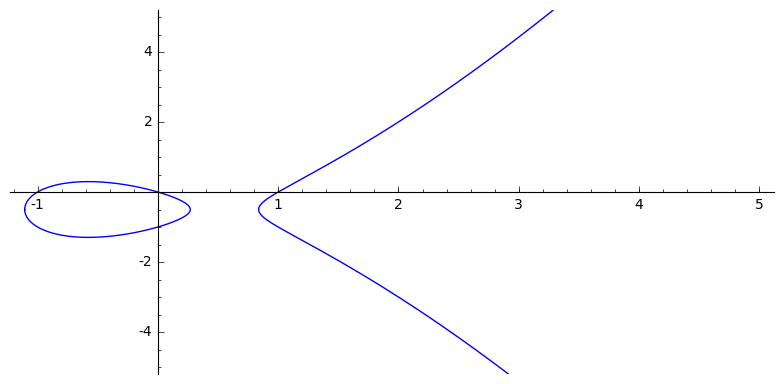
\includegraphics[scale=0.6]{normcurve}
%
%We want to disregard curves which have cusps, self-intersections, or isolated points (which together are called singularities), as we want to be able to create a unique tangent line given any point. We want to find an easily checkable algebraic property which defines these bad cases, instead of a geometric one.
%
%Note that the elliptic curve can also be described as the roots of this function:
%
%$$E(x,y) = y^2 - x^3 - ax - b$$
%
%Note that singular points all imply that $\nabla E(x,y) = 0$ at these bad points.
%
%$$\nabla E(x,y) = (-3x^2-a,2y)$$
%
%So we have
%
%$$y=0$$
%$$3x^2+a=0$$
%$$ y^2 = x^3 + ax + b$$
%
%That hold for all bad curves. This system of equations can be solved using elementary methods.
%
%$$3x^2 = -a$$
%
%$$\begin{aligned} x^3 + ax + b &= 0\\
% (x^3 + ax)^2 &= b^2\\
% x^6 + 2ax^4+a^2x^2 &= b^2\\
% 27x^6 + 27\times2ax^4+ 27a^2x^2 &= 27b^2\\
% (3x^2)^3 + 6 a (3x^2)^2+ 9a^2(3x^2) &= 27b^2\\
% (-a)^3 + 6a (-a)^2+ 9a^2(-a) &= 27b^2\\
% -a^3 + 6a^3- 9a^3 &= 27b^2\\
% -4a^3 &= 27b^2\\
% 4a^3+27b^2 &= 0\\
% \end{aligned}$$
%
%So we found our condition: $4a^3 + 27b^2 \ne 0$ implies there will be no singularities points, and so there will always be a tangent line to a point. Any curve of the elliptic form for which the condition does not hold is not defined to be an elliptic curve.
%
%\subsection{Elliptic Group law}
%
%Operating in the projective plane of the curve, which is $(\ZMZ{n})^2$, in the context of primality proving, you can define a group operation, written as $+$. However, you need to define an extra point on the plane, which serves as the identity of the group. Call it $\OS$. This can be thought of as the point at infinity. It is also often notated as $0$ or $\infty$.
%
%The group law holds as follows. Take 2 points $P, Q$ that lie on the curve. Find the 3rd point, $R$, on the curve which also lies on that line. Then $P+Q+R = \OS$ (GRAPHIC HERE!!!!).
%
%\subsection{Geometric Construction of the Group Operation}
%
%Keeping that law in mind, what we want to know is how to construct $P+Q$ so that the law holds.
%
%Now, if $y_P = y_Q$, and $P \ne Q$, then there is no third point along curve on the line connecting P and Q on the ordinary plane (this fact relates to quadratics only having 2 roots). But if $y_P = y_Q+\Delta$, with $|\Delta|$ small, then $y_R$ will be very large.
%
%Here is a zoomed out version of the same elliptic curve so that  you can see its behavior as it approaches infinity.
%
%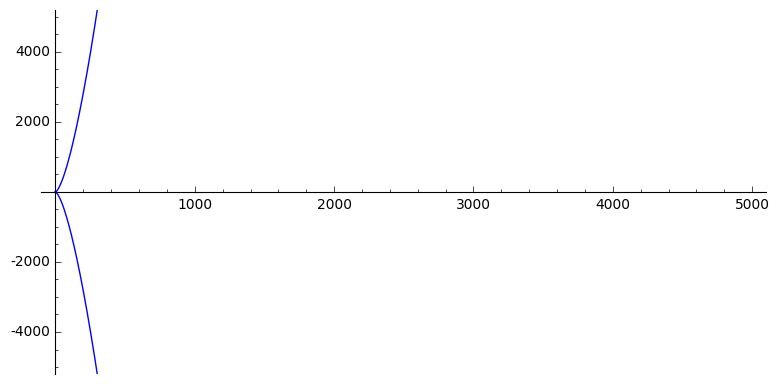
\includegraphics[scale=0.6]{backscaled}
%
%So $P+Q$ is defined to be the point at infinity, $O$. Notice that we just found the additive inverse, $-P = (x_P,-y_P)$.
%
%Another way of thinking about this is examining of which lines through the curve have no 3rd point. After careful examination, it is only points which are tangent to the curve, which are taken care of separately below, or those which
%
%By the above group law, $P+Q = -R$, so to summarize, if we draw a point between $P$ and $Q$, $P+Q$ is the 3rd point on the line, flipped over the $X$ axis.
%
%In the cases of lines being tangent to the line at a point, think of the point being almost tangent to the curve, so that it actually intersects the curve at two points, which happen to lie so close together that they are actually the same point. So, if the line between $P$ and $Q$ is the tangent line to $P$, then $-(P+Q)=P$.(GRAPHIC of THIS). $P+P=Q$, where $Q$ is the 3rd item on the tangent
%
%\subsection{Algebraic Construction of the Group Operation}
%
%This geometric intuition can be turned into an equivalent algebraic definition, which is better to work with the algebraic proofs involving primality, and translates better to finite fields.
%
%Let $P = (x_P,y_P), Q = (x_Q,y_Q)$. Assuming $x_P \ne x_Q$, $s$, the slope between $P$ and $Q$, can be calculated,
%
%$$s = \frac{y_P - y_Q}{x_P - x_Q}$$
%
%Now, considering $x_P = x_Q$. If $y_P = y_Q$, then $R$ is defined to be 0. Otherwise,
%
%We can see that $R = (P+Q)$ is just
%
%$$x_R = s^2 - x_P - x_Q$$
%
%$$y_R = y_P + s(x_R - x_P)$$
%
%\section{Factorization Using Elliptic Curves}
%
%
%
%\section{Hasse's theorem}
%
%If $n$ is the number of points on the elliptic curve $E$ over a finite field with $q$ elements, then
%
%$$|N - (q+1)| \le 2\sqrt{q}$$
%
%\section{Pocklington Criterion}
%
%Let $N \in \Z, N > 1$, suppose there exists $a$.
%
%\section{Elliptic curve primality criterion}
%
%Source:
%
%http://theory.stanford.edu/~dfreeman/cs259c-f11/finalpapers/primalityproving.pdf
%
%
%Let $n$ be an integer not dividible by 2 or 3. Let $A,B \in \Z_n$ ushc that $(4A^3 + 27B^2,n) = 1$, and let $L \ne E_{A,B}(\Z_n)$. If there exists a prime $q > (\sqrt[4]{n} + 1)^2$ such that $qL = \OS$, then $n$ is prime.
%
%\subsection{Proof 1}
%
%By contraditction. Suppose $n$ is composite. Then there exists a prime $o > 3$ dividing $n$, so that $p \ne \sqrt{n}$. Note that $4a^3 + 27B^2 \ne 0 (mod\ p)$ or else
%
%Let $N \in \Z, N  >0$, and let E be the set defined by $y^2 = x^3 + ax + b ($mod $ N)$.
%
%Now let $m$ be an integer. If there is a prime $q$ which divides $m$, and is greater than $(N^{1/4} + 1)^2$, and there exists a point $p$ on $E$ such that
%
%\section{Factoring Overview}
%
%Primality testing using elliptic curves was inspired by factoring methods, so I will lay out the factoring methods here to give more intuition for the more difficult primality testing methods.
%
%\subsection{$p-1$ factoring}
%
%%http://www.math.mcgill.ca/darmon/courses/05-06/usra/charest.pdf
%
%Elliptic curve factoring closely mirrors Pollard's $p-1$ algorithm.
%
%%This argument is aufully structural, any exmplanation will need to be very, very careful.
%%Let $n$ be a composite integer. Let $pl=n$, where $p$ is the some unknown prime, and $l$ is some integer. We want to use the fact that for $x$ coprime to $n$, $(\ZMZ{n})^* = (\ZMZ{p})^*$ is multiplicatively cyclic with order $p-1$. In particular, we can check
%
%The basic idea of how to do this: Choose a random $x \in \ZMZ{n}$. Choose an $m=1,2,3,...,n$ and compute $x^m$ until $x^m - 1 | p$. By Fermat's little theorem, this will always occur at $m=p-1$, unless $x|p$. We can check if $x^m - 1 | p$ even though we don't know $p$, because  $\gcd(x^m-1,n=pl)$ will be $p$, instead of 1. By Fermat's little theorem,  The problem is that this is really slow, because we have to raise $x^m$, $p-1$ times, which is no faster than trial and error factorization. There are ways to speed this up without elliptic curves, but instead of going into detail on these, I will move on to elliptic curve factoring to speed this basic idea up.
%
%Noting that by Fermat's little theorem. For $a \nmid p$ and $K > 0$,
%
%$$a^{K(p-1)} = (a^{(p-1)})^K = 1^K = 1 \Mod{p}$$
%
%So instead of choosing $m$ one at a time, we can choose an $m=B!$, where we $B >= p-1$, but $B < q-1$, where $q$ is the largest prime factor of $n$. We like $m$ because
%
%\subsection{Elliptic curve factoring}
%
%Elliptic curve factoring closely mirrors $p-1$ factoring in two main ways. Instead of choosing an $x$ in $(\ZMZ{n})^*$, we choose $\pi \in E(\ZMZ{n})$. Then, as $E(\ZMZ{n})$ is additive instead of multiplicative like $(\ZMZ{n})^*$, we start multiplying $\pi$ by increasing values of $m$, instead of raising it to  powers. So instead of looking for a power of $x$ that gives the multiplicative identity $\Mod{p}$, 1, we look for failed invertibility $\Mod{n}$
%
%Recalling the formulas for elliptic point addition, we can check if $x=\OS$ because our calculation of the slope of the line will fail because of division by zero, effectively giving back infinity.
%
%\[
%m = \left\{\begin{array}{lr}
%\frac{y_2-y_1}{x_2-x_1}, & \text{if } x_1 \ne x_2 \\
%\frac{3x_1^2+a}{2y_1}, & \text{if } x_1 = x_2
%\end{array}\right\}
%\]
%
%You can see that division by zero happens when
%
%We really only start looking at elliptic curves when trying to find the value of $p$. Instead of using the condition $\gcd(a^m - 1,pl=n)$, to find $p$, inspired by Fermat's little theorem, we examine the that $m = $
%

\end{document}
